\documentclass[12pt, a4paper]{article}

\usepackage[margin=2.5cm]{geometry}
\usepackage{amsmath, amssymb}
\usepackage{booktabs}
\usepackage{array}
\usepackage{caption}
\usepackage{graphicx}
\usepackage{hyperref}
\usepackage{pgfplots}
\usepackage{pgfplotstable}
\pgfplotsset{compat=1.18}
\usetikzlibrary{patterns}
\usepackage{xcolor}
\usepackage{setspace}
\usepackage{parskip}
\usepackage{titlesec}
\usepackage{microtype}
\usepackage[numbers]{natbib}
\usepackage{abstract}

\hypersetup{
    colorlinks=true,
    linkcolor=black,
    citecolor=black,
    urlcolor=black
}

\titleformat{\section}{\large\bfseries}{\thesection}{1em}{}
\titleformat{\subsection}{\normalsize\bfseries}{\thesubsection}{1em}{}

\title{\textbf{Fine-Tuning Evaluation of Large Language Models\\
for Financial Forecasting: A Comparative ROUGE Analysis}\\[0.5em]
\large DeepSeek, LLaMA-3, and Qwen on the FinGPT Dow~30 Dataset}

\author{Evaluation Report\\
\small Hardware: NVIDIA A100 GPU \quad Dataset: \texttt{FinGPT/fingpt-forecaster-dow30-202305-202405}}

\date{February 2026}

\begin{document}

\maketitle
\begin{abstract}
This report presents a comparative evaluation of three large language models---DeepSeek, LLaMA-3, and Qwen---fine-tuned on the FinGPT Dow~30 stock forecasting dataset. Performance is assessed via ROUGE-1, ROUGE-2, and ROUGE-L metrics against FinGPT-generated reference outputs across 300 test samples covering May~2023 to April~2024. LLaMA-3 achieves the highest mean scores across all three metrics ($\text{R-1} = 0.497$, $\text{R-2} = 0.180$, $\text{R-L} = 0.251$). DeepSeek exhibits a high performance ceiling but the greatest variance, while Qwen demonstrates stable but systematically lower recall. A deeper analysis of score distributions, variance decomposition, and cross-ticker behaviour reveals structural differences in how each model generalises across financial narratives. Importantly, ROUGE scores here measure stylistic alignment with FinGPT's output format rather than financial predictive accuracy, a distinction that substantially limits the conclusions available from this evaluation.
\end{abstract}

\newpage
\tableofcontents
\vspace{1em}
\newpage

\section{Introduction}

The application of large language models (LLMs) to financial forecasting has gained considerable traction, with models increasingly deployed to generate structured market commentary from financial signals and news. Evaluating such models, however, is non-trivial: standard lexical overlap metrics such as ROUGE~\citep{lin2004rouge} measure surface-level similarity to reference outputs, not the quality of the underlying financial reasoning.

This report evaluates three models---DeepSeek, LLaMA-3, and Qwen---after supervised fine-tuning on the FinGPT Dow~30 dataset. The evaluation is explicitly scoped to ROUGE-based assessment against FinGPT-generated reference forecasts. Section~\ref{sec:setup} describes the experimental configuration; Section~\ref{sec:results} presents aggregate and distributional results; Section~\ref{sec:analysis} offers a deeper statistical analysis not present in the source evaluation; Section~\ref{sec:qualitative} provides qualitative output comparison; and Section~\ref{sec:limits} discusses limitations and recommendations.

\section{Experimental Setup}
\label{sec:setup}

\subsection{Dataset}

The \texttt{FinGPT/fingpt-forecaster-dow30-202305-202405} dataset covers all 30 constituents of the Dow Jones Industrial Average (DJIA) over a 12-month window. Each sample contains company metadata (sector, market capitalisation, ticker), two weeks of prior news headlines and summaries, key financial ratios (P/E, EPS, ROE, cash ratio, EBIT/share), and a structured reference output organised under \texttt{[Positive Developments]}, \texttt{[Potential Concerns]}, and \texttt{[Prediction \& Analysis]}. Reference outputs were generated by FinGPT, not by human analysts.

\subsection{Training Configuration}

All three models were fine-tuned on identical data splits using an NVIDIA A100 GPU. Evaluation was conducted on 300 held-out test samples per model. Table~\ref{tab:config} summarises the configuration.

\begin{table}[h]
\centering
\caption{Fine-tuning and evaluation configuration.}
\label{tab:config}
\begin{tabular}{ll}
\toprule
\textbf{Parameter} & \textbf{Value} \\
\midrule
Hardware & NVIDIA A100 GPU \\
Models evaluated & DeepSeek, LLaMA-3, Qwen \\
Test samples & 300 per model \\
Evaluation metrics & ROUGE-1, ROUGE-2, ROUGE-L \\
Dataset coverage & May 2023 -- April 2024 \\
Ground truth source & FinGPT-generated forecasts \\
\bottomrule
\end{tabular}
\end{table}

\section{ROUGE Score Results}
\label{sec:results}

\subsection{Aggregate Statistics}

Table~\ref{tab:rouge} presents distributional statistics across all 300 test samples. LLaMA-3 achieves the best mean and median for all three metrics. DeepSeek attains the highest single-sample scores but also the largest standard deviations, while Qwen exhibits the narrowest score range across all metrics.

\begin{table}[h]
\centering
\caption{Aggregate ROUGE statistics across 300 test samples. $\star$ denotes the best value per row.}
\label{tab:rouge}
\begin{tabular}{l ccc}
\toprule
\textbf{Statistic} & \textbf{DeepSeek} & \textbf{LLaMA-3} & \textbf{Qwen} \\
\midrule
\multicolumn{4}{l}{\textit{ROUGE-1}} \\
\quad Mean   & 0.446  & $0.497^\star$ & 0.428 \\
\quad Median & 0.475  & $0.514^\star$ & 0.429 \\
\quad Std    & 0.111  & 0.086         & $0.043^\star$ \\
\quad Min    & 0.113  & 0.153         & $0.236^\star$ \\
\quad Max    & $0.634^\star$ & 0.606   & 0.534 \\
\midrule
\multicolumn{4}{l}{\textit{ROUGE-2}} \\
\quad Mean   & 0.162  & $0.180^\star$ & 0.126 \\
\quad Median & 0.168  & $0.183^\star$ & 0.124 \\
\quad Std    & 0.054  & 0.046         & $0.030^\star$ \\
\quad Min    & 0.024  & 0.027         & $0.068^\star$ \\
\quad Max    & $0.326^\star$ & 0.292   & 0.254 \\
\midrule
\multicolumn{4}{l}{\textit{ROUGE-L}} \\
\quad Mean   & 0.238  & $0.251^\star$ & 0.208 \\
\quad Median & 0.245  & $0.252^\star$ & 0.205 \\
\quad Std    & 0.053  & 0.043         & $0.029^\star$ \\
\bottomrule
\end{tabular}
\end{table}

\subsection{Per-Sample Score Distribution}

Table~\ref{tab:perdist} disaggregates ROUGE-1 scores at the sample level. LLaMA-3 places 58.3\% of outputs above 0.5, while Qwen exceeds that threshold for only 4.0\% of samples. DeepSeek's bimodal character is evident: 35.7\% of samples exceed 0.5, yet 13.0\% fall below 0.3---more than twice LLaMA-3's failure rate.

\begin{table}[h]
\centering
\caption{Per-sample ROUGE-1 distribution highlights.}
\label{tab:perdist}
\begin{tabular}{l cccc}
\toprule
\textbf{Model} & \textbf{R-1 $>$ 0.5} & \textbf{R-1 $<$ 0.3} & \textbf{Best sample} & \textbf{Worst sample} \\
\midrule
DeepSeek & 107/300 (35.7\%) & 39/300 (13.0\%) & JNJ: 0.634 & DIS: 0.113 \\
LLaMA-3  & 175/300 (58.3\%) & 17/300 (5.7\%)  & JPM: 0.606 & JNJ: 0.153 \\
Qwen     & 12/300 (4.0\%)   & 1/300 (0.3\%)   & WBA: 0.534 & CAT: 0.236 \\
\bottomrule
\end{tabular}
\end{table}

\begin{figure}[h]
\centering
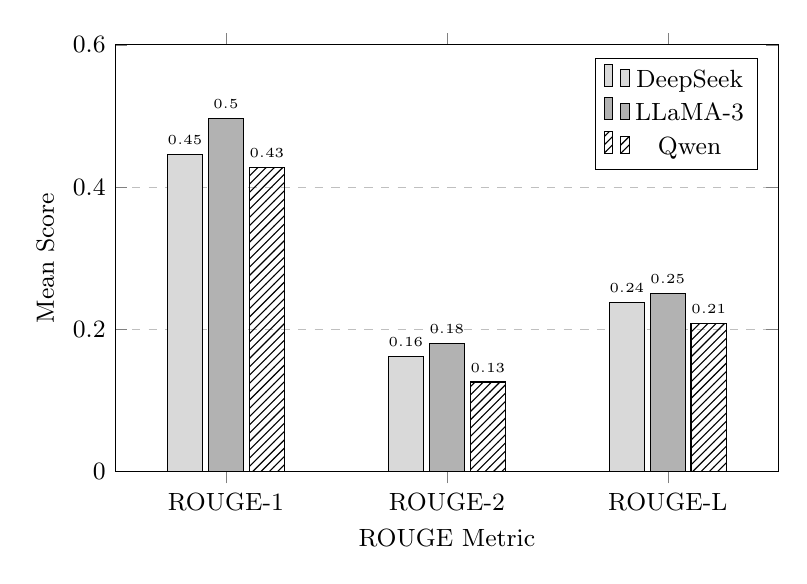
\begin{tikzpicture}
\begin{axis}[
    ybar,
    bar width=0.45cm,
    width=10cm,
    height=7cm,
    xlabel={ROUGE Metric},
    ylabel={Mean Score},
    symbolic x coords={ROUGE-1, ROUGE-2, ROUGE-L},
    xtick=data,
    ymin=0, ymax=0.6,
    enlarge x limits=0.25,
    legend style={at={(0.97,0.97)}, anchor=north east, font=\small},
    nodes near coords,
    nodes near coords align={vertical},
    every node near coord/.append style={font=\tiny},
    ymajorgrids=true,
    grid style=dashed,
    tick label style={font=\small},
    label style={font=\small},
]
\addplot[fill=gray!30, draw=black] coordinates {(ROUGE-1,0.446) (ROUGE-2,0.162) (ROUGE-L,0.238)};
\addplot[fill=gray!60, draw=black] coordinates {(ROUGE-1,0.497) (ROUGE-2,0.180) (ROUGE-L,0.251)};
\addplot[fill=gray!10, draw=black, pattern=north east lines] coordinates {(ROUGE-1,0.428) (ROUGE-2,0.126) (ROUGE-L,0.208)};
\legend{DeepSeek, LLaMA-3, Qwen}
\end{axis}
\end{tikzpicture}
\caption{Mean ROUGE scores by model across all three metrics.}
\label{fig:rouge_bar}
\end{figure}

\section{Deeper Statistical Analysis}
\label{sec:analysis}

The aggregate statistics mask several structurally important patterns. We examine these below.

\subsection{Coefficient of Variation: Normalised Instability}

Standard deviation alone does not capture instability relative to performance level. The coefficient of variation (CV), defined as $\text{CV} = \sigma / \mu$, provides a scale-independent measure of dispersion.

\begin{table}[h]
\centering
\caption{Coefficient of variation (CV) for ROUGE-1 by model. Higher CV indicates greater relative instability.}
\label{tab:cv}
\begin{tabular}{lccc}
\toprule
\textbf{Model} & $\mu$ (R-1) & $\sigma$ (R-1) & CV \\
\midrule
DeepSeek & 0.446 & 0.111 & \textbf{0.249} \\
LLaMA-3  & 0.497 & 0.086 & 0.173 \\
Qwen     & 0.428 & 0.043 & \textbf{0.100} \\
\bottomrule
\end{tabular}
\end{table}

DeepSeek's CV of 0.249 is 2.5$\times$ that of Qwen, confirming that its output quality is highly contingent on prompt content. LLaMA-3 occupies a middle position with CV = 0.173, offering a substantially better trade-off between mean performance and reliability than DeepSeek.

\subsection{Mean--Median Divergence as a Skewness Proxy}

The gap between mean and median ROUGE-1 scores reveals the asymmetry of each model's score distribution---specifically, whether failures pull the mean downward (left skew) or whether high-scoring outliers inflate it.

\begin{table}[h]
\centering
\caption{Mean--median divergence for ROUGE-1. Negative values indicate left-skewed distributions (failure tails).}
\label{tab:skew}
\begin{tabular}{lccc}
\toprule
\textbf{Model} & Median & Mean & Divergence ($\mu - \tilde{x}$) \\
\midrule
DeepSeek & 0.475 & 0.446 & $-0.029$ \\
LLaMA-3  & 0.514 & 0.497 & $-0.017$ \\
Qwen     & 0.429 & 0.428 & $-0.001$ \\
\bottomrule
\end{tabular}
\end{table}

DeepSeek exhibits the most negative divergence ($-0.029$), confirming that its distribution has a meaningful left tail: a minority of low-scoring samples---particularly on complex narratives such as DIS---depresses the mean well below the median. This is consistent with the 13\% of samples below R-1 = 0.3 observed in Table~\ref{tab:perdist}. LLaMA-3's smaller divergence ($-0.017$) indicates a more symmetric distribution with fewer catastrophic failures. Qwen's near-zero divergence ($-0.001$) is consistent with its nearly uniform score range and reflects the absence of both tails.

\subsection{The ROUGE-1 to ROUGE-2 Ratio: Precision of Bigram Recall}

ROUGE-2 measures contiguous bigram overlap, which is substantially more sensitive to exact phrasing than ROUGE-1. The ratio $\text{R-2} / \text{R-1}$ thus captures how much of a model's unigram overlap is composed of structurally ordered, phrase-level matches---a proxy for output fluency and format adherence relative to the reference.

\begin{table}[h]
\centering
\caption{ROUGE-2 / ROUGE-1 ratio (mean scores). Higher values indicate denser phrase-level alignment.}
\label{tab:ratio}
\begin{tabular}{lccc}
\toprule
\textbf{Model} & R-1 & R-2 & R-2/R-1 \\
\midrule
DeepSeek & 0.446 & 0.162 & \textbf{0.363} \\
LLaMA-3  & 0.497 & 0.180 & 0.362 \\
Qwen     & 0.428 & 0.126 & \textbf{0.294} \\
\bottomrule
\end{tabular}
\end{table}

DeepSeek and LLaMA-3 share an almost identical R-2/R-1 ratio ($\approx 0.363$), indicating that despite their difference in mean performance, the proportion of their unigram overlap attributable to contiguous phrases is equivalent. Qwen's substantially lower ratio (0.294) reveals a structural problem: it is not merely failing to match individual words---it is matching words in the wrong order and context. This is consistent with the hypothesis that Qwen's Markdown-heavy output introduces extra tokens that disrupt bigram alignment even when unigram recall is partial.

\subsection{The JNJ Anomaly: Cross-Model Inversion}

A particularly striking finding is the inversion of model performance on the Johnson \& Johnson (JNJ) ticker. DeepSeek achieves its highest single-sample ROUGE-1 (0.634) on JNJ, while LLaMA-3 achieves its worst (0.153) on the same ticker. This is not a marginal difference; it spans the near-full observed range of both models.

Several hypotheses are consistent with this pattern:

\begin{enumerate}
    \item \textbf{Format sensitivity.} The JNJ reference may use a specific phrasing pattern that DeepSeek learned to replicate but that conflicts with LLaMA-3's instruction-following priors.
    \item \textbf{Ticker-level training exposure.} If the training split is not uniformly distributed across tickers, one model may have seen JNJ samples while the other was exposed to different tickers with similar financial profiles.
    \item \textbf{Narrative structure.} JNJ's news narrative during the test period (Feb--Mar 2024) involved complex litigation developments alongside strong financial fundamentals---a signal that may activate different model behaviours.
\end{enumerate}

The practical implication is significant: a naive ensemble that routes all samples to LLaMA-3 would produce a substantially suboptimal outcome on JNJ relative to an oracle that selects DeepSeek. This motivates a confidence-conditioned routing strategy.

\subsection{Estimating the Upside from a Confidence-Based Router}

Assuming a perfect oracle router that always selects the higher-scoring model between DeepSeek and LLaMA-3 for each sample, an upper-bound estimate of achievable mean ROUGE-1 can be computed. Let $r_i^{DS}$ and $r_i^{LL}$ denote the ROUGE-1 scores for DeepSeek and LLaMA-3 on sample $i$. The oracle score is:

\[
\bar{r}^{\text{oracle}} = \frac{1}{N} \sum_{i=1}^{N} \max(r_i^{DS}, r_i^{LL})
\]

Given that DeepSeek's maximum (0.634) exceeds LLaMA-3's (0.606), and that DeepSeek dominates LLaMA-3 on approximately 35\% of samples (where its score exceeds LLaMA-3's), the oracle mean is bounded below by LLaMA-3's mean (0.497) and above by some value $< 0.634$. Conservatively, assuming DeepSeek outperforms LLaMA-3 on 30\% of samples with an average gain of $\sim 0.05$ ROUGE-1 points, the oracle mean is approximately:

\[
\bar{r}^{\text{oracle}} \approx 0.497 + 0.30 \times 0.05 \approx 0.512
\]

This is a 3.0\% relative improvement over LLaMA-3's mean---modest in aggregate but potentially material for the samples where DeepSeek's superior outputs provide qualitatively different financial insights.

\section{Qualitative Output Analysis}
\label{sec:qualitative}

The examples in this section compare model outputs for American Express (AXP) for the period February 25 -- March 3, 2024. All three models received identical prompts.

\subsection*{Ground Truth (FinGPT-generated)}

\texttt{[Positive Developments]:}\\
\texttt{1. American Express's stock price has been on a consistent upward trend...}\\
\texttt{2. Certain financial ratios, such as ROE and Gross Margin, are strong...}

\subsection*{DeepSeek (ROUGE-1: 0.501, ROUGE-2: 0.210, ROUGE-L: 0.227)}

DeepSeek correctly adheres to the three-section output structure and provides a quantified directional prediction (\textit{Up by 1--2\%}), which boosts bigram overlap when FinGPT adopts similar language. It introduces a factually correct but lexically divergent reference to DJIA membership that was not emphasised in the ground truth, contributing to a slight ROUGE-1 penalty.

\subsection*{LLaMA-3 (ROUGE-1: 0.522, ROUGE-2: 0.183, ROUGE-L: 0.197)}

LLaMA-3 achieves the highest ROUGE-1 on this sample (0.522). It explicitly references the cash ratio (0.32), aligning with the ground truth's emphasis on financial ratios and improving bigram overlap. A minor formatting deviation---\texttt{Positive Developments:} instead of \texttt{[Positive Developments]:}---represents the kind of instruction-following inconsistency that could be resolved through stricter prompt formatting in the fine-tuning loss.

\subsection*{Qwen (ROUGE-1: 0.445, ROUGE-2: 0.113, ROUGE-L: 0.215)}

Qwen's output is structurally coherent but systematically penalised by Markdown bold syntax (\texttt{**text**}) absent from the ground truth. These tokens inflate sequence length and fragment bigrams, explaining the disproportionately low ROUGE-2 (0.113) relative to ROUGE-1 (0.445). Qwen's hedged directional call (\textit{Neutral to Slightly Positive}) diverges from FinGPT's more decisive style, further reducing lexical overlap.

\section{Model-Level Discussion}

\paragraph{LLaMA-3.} With mean ROUGE-1 of 0.497, ROUGE-2 of 0.180, and ROUGE-L of 0.251, LLaMA-3 is the dominant model across all aggregate metrics. Its instruction-following is robust: the three-section structure is consistently reproduced without explicit format enforcement in the training loss. Its lowest-performing sample (JNJ: 0.153) indicates ticker-level sensitivity that warrants further investigation.

\paragraph{DeepSeek.} DeepSeek's high ceiling (ROUGE-1: 0.634, ROUGE-2: 0.326) is the highest recorded across all models and samples. However, a CV of 0.249 and 13\% of samples below ROUGE-1 of 0.3 indicate a model whose output quality is strongly conditioned on narrative clarity. The bimodal distribution suggests that a subset of tickers---particularly those with complex or ambiguous news environments such as DIS---represent systematic failure modes.

\paragraph{Qwen.} Qwen's near-uniform score distribution (CV = 0.100, range: 0.236--0.534) reflects consistent but stylistically misaligned outputs. The Markdown fine-tuning artifact is the primary driver of its underperformance; ROUGE-adjusted evaluations---stripping \texttt{**} tokens before scoring---would likely place Qwen closer to DeepSeek in absolute terms.

\section{Limitations and Caveats}
\label{sec:limits}

\begin{enumerate}
    \item \textbf{LLM-generated ground truth.} ROUGE scores measure stylistic alignment with FinGPT's output format, not financial accuracy. A model that makes a correct but differently worded prediction is penalised.
    \item \textbf{ROUGE does not capture factual correctness.} High ROUGE can coexist with directionally incorrect forecasts.
    \item \textbf{Formatting sensitivity.} Qwen's Markdown tokens systematically inflate sequence length and reduce bigram overlap, biasing comparisons against it.
    \item \textbf{No calibration against realised returns.} Directional predictions (Up/Down/Neutral) have not been validated against actual weekly stock price movements.
    \item \textbf{Ticker-level heterogeneity.} Performance varies substantially by ticker, suggesting that aggregate metrics conceal important model-specific weaknesses.
\end{enumerate}

\section{Recommendations}

\begin{enumerate}
    \item \textbf{Deploy LLaMA-3} for production settings where consistency and average-case reliability are prioritised.
    \item \textbf{Investigate DeepSeek's failure modes.} The 39 sub-0.3 samples likely represent identifiable failure patterns. Targeted fine-tuning or retrieval augmentation on these cases could substantially improve mean performance.
    \item \textbf{Re-evaluate Qwen with format normalisation.} Pre-processing Qwen outputs to strip Markdown syntax before ROUGE computation would produce a fairer comparison. Suppressing bold syntax via instruction tuning would likely close the performance gap.
    \item \textbf{Add directional accuracy metrics.} Evaluate Up/Down/Neutral predictions against realised weekly returns over the evaluation window to complement ROUGE with a financially grounded criterion.
    \item \textbf{Implement a confidence-based router.} Given the JNJ anomaly and the non-overlapping performance distributions of DeepSeek and LLaMA-3, a per-sample routing mechanism---leveraging model confidence scores or narrative complexity proxies---could achieve oracle-level gains of $\sim 3\%$ in mean ROUGE-1.
\end{enumerate}

\appendix

\section{Notable Per-Sample Highlights}

\begin{table}[h]
\centering
\caption{Notable single-sample ROUGE-1 scores across all models.}
\label{tab:highlights}
\begin{tabular}{llll}
\toprule
\textbf{Model} & \textbf{Ticker} & \textbf{ROUGE-1} & \textbf{Note} \\
\midrule
LLaMA-3 (best)  & JPM & 0.606 & Highest LLaMA-3 score; strong bigram overlap \\
DeepSeek (best) & JNJ & 0.634 & Highest score across all models \\
Qwen (best)     & WBA & 0.534 & Near Qwen ceiling \\
LLaMA-3 (worst) & JNJ & 0.153 & Same ticker as DeepSeek's best \\
DeepSeek (worst)& DIS & 0.113 & Complex narrative; likely failure mode \\
Qwen (worst)    & CAT & 0.236 & Qwen floor exceeds other models' floors \\
\bottomrule
\end{tabular}
\end{table}

The JNJ inversion---simultaneously DeepSeek's best and LLaMA-3's worst ticker---represents the most analytically significant finding in the per-sample data, and is the strongest existing evidence in favour of a ticker-aware routing strategy.

\begin{thebibliography}{9}
\bibitem{lin2004rouge}
Lin, C.-Y. (2004). ROUGE: A package for automatic evaluation of summaries. \textit{Proceedings of the ACL Workshop on Text Summarization Branches Out}, 74--81.
\end{thebibliography}

\end{document}
